\documentclass[t,dvipsnames]{beamer}
\usepackage{amsmath}
\usepackage{siunitx}
\usepackage[T1]{fontenc}
\usepackage[sfdefault,lining,scaled=.85]{FiraSans}
\usepackage[scaled=0.85]{FiraMono}
\usepackage{newtxsf}
\usepackage{pifont}
\usepackage[utf8]{inputenc}
\usepackage{mdwlist}
\usepackage{hyperref}

\usetheme{UAmnf}

\setbeamerfont{frametitle}{family=\sffamily\firamedium}
\setbeamercolor{frametitle}{fg=white}
\setbeamertemplate{navigation symbols}{}
\setbeamertemplate{headline}{  
  \leavevmode
   \begin{beamercolorbox}{logo in headline}
	\includegraphics[width=\paperwidth]{UA_mnf_headline}
   \end{beamercolorbox}
}
\setbeamercolor{alerted text}{fg=red!70!black}

\hypersetup{%
  pdftitle={Introduction to Feynman path integrals}
  ,pdfauthor={Gert-Ludwig Ingold}
  ,pdfsubject={Presentation at the Bad Honnef Physics School on
	       Methods of Path Integration in Modern Physics, Bad Honnef, 25.8.2019}
  ,pdfkeywords={Feynman path integrals, propagator, particle in a box,
                particle on a ring, harmonic oscillator}
}

\graphicspath{{./img/}}

\title[Introduction to Feynman path integrals]%
      {Introduction to Feynman path integrals}

\begin{document}

\begin{frame}[t]{}
 \vspace{2.0truecm}
 \begin{center}
   \structure{\LARGE\firamedium Introduction to Feynman path integrals}\\[0.2truecm]

   \vspace{0.1truecm}
   {\Large Gert-Ludwig Ingold}

   {\large Universität Augsburg}

   \vspace{3.4truecm}
   {\scriptsize Bad Honnef Physics School on \textit{Methods of Path Integration in
    Modern Physics}, 25.--31.8.2019}
 \end{center}
\end{frame}

\navtrue

\section{Motivation}

\begin{frame}[c]{}
 \begin{center}
  \begin{minipage}{0.8\textwidth}
   \only<1>{\tableofcontents}%
   \only<2>{\tableofcontents[currentsection]}%
  \end{minipage}
 \end{center}
\end{frame}

\begin{frame}[t]{Classical mechanics: Hamilton vs. Lagrange}

 \vspace{-0.5truecm}
 \begin{columns}
  \begin{column}[t]{0.5\textwidth}
   \begin{center}
    \textbf{Hamilton formalism}

    Hamiltonian $H(q, p)$

    \vspace{0.2truecm}
    Poisson bracket $\{q, p\} = 1$

    equations of motion $\dot q = \{q, H\}, \dot p = \{p, H\}$
   \end{center}
  \end{column}%
  \begin{column}[t]{0.5\textwidth}
   \begin{center}
    \textbf{Lagrange formalism}

    Lagrangian $L(q, \dot q)$

    \vspace{0.2truecm}
    action $S = \int\text{d}t L(q, \dot q)$

    equation of motion from Hamilton's principle $\delta S = 0$

   \end{center}
  \end{column}%
 \end{columns}

 \begin{columns}
  \begin{column}[t]{0.5\textwidth}
   \begin{center}
    $\Arrowvert$

    canonical quantization $[\hat q, \hat p] = \text{i}\hbar$

    $\Downarrow$
   \end{center}
  \end{column}%
  \begin{column}[t]{0.5\textwidth}
   \begin{center}
    $\Arrowvert$

    ?

    $\Downarrow$
   \end{center}
  \end{column}%
 \end{columns}

 \begin{columns}
  \begin{column}[t]{0.5\textwidth}
   \begin{center}
   Heisenberg, Schrödinger, \ldots (1925)

   Schrödinger equation $\hat H\vert\Psi\rangle =
	  \text{i}\hbar\frac{\partial}{\partial t}\vert\Psi\rangle$ 
   \end{center}
  \end{column}%
  \begin{column}[t]{0.5\textwidth}
   \begin{center}
    Dirac (1933), Feynman (1948)

    \vspace{0.2truecm}
    \fcolorbox{red!70!black}{red!10}{%
       \begin{minipage}{0.75\textwidth}
	\begin{center}
         \alert{Path integral formulation of quantum mechanics}
	\end{center}
       \end{minipage}
    }
   \end{center}
  \end{column}%
 \end{columns}
\end{frame}

\begin{frame}[c]{Why base quantum mechanics\\ on Lagrange formalism?}
 path integral formulation of quantum mechanics \ldots
 \begin{itemize}
  \item \ldots can provide an alternative view on physical problems
  \item \ldots does without operators\\
	for fermionic fields, Grassmann variables are used
  \item \ldots is very well suited for relativistic field theories\\[0.2truecm]
	action $S=\int\text{d}^4x\mathcal{L}(\phi, \partial_\mu\phi)$
		 is a Minkowski scalar\\[0.2truecm]
	Hamiltonian density $\mathcal{H}(\phi, \pi)$ corresponds to the
	$0-0$ component of the energy-momentum tensor
  \item \ldots is very well suited to consider the semiclassical limit
	$S\gg\hbar$
 \end{itemize}
\end{frame}

\section{Propagator}

\begin{frame}[c]{}
 \begin{center}
  \begin{minipage}{0.8\textwidth}
   \tableofcontents[currentsection]
  \end{minipage}
 \end{center}
\end{frame}

\begin{frame}[t]{Propagator}
 Schrödinger equation\quad
 $\text{i}\hbar\dfrac{\partial}{\partial t}\vert\Psi(t)\rangle = H\vert\Psi(t)\rangle$

 \vspace{0.5truecm}
 time evolution of a state
 \begin{displaymath}
  \vert\Psi(t)\rangle = U(t)\vert\Psi(0)\rangle\quad \text{with}\quad
  U(t) = \exp\left(-\frac{\text{i}}{\hbar}Ht\right)
 \end{displaymath}
 in position representation
 \begin{displaymath}
  \textcolor{blue}{\langle q_\text{f}}\vert\Psi(t)\rangle =
   \textcolor{green!40!black}{\int\!\!\text{d}q_\text{i}}\textcolor{blue}{\langle q_\text{f}\vert}
   U(t)\textcolor{green!40!black}{\vert q_\text{i}\rangle\langle q_\text{i}}\vert\Psi(0)\rangle
 \end{displaymath}
 \begin{displaymath}
  \Psi(q_\text{f}, t) = \int\text{d}q_\text{i} K(q_\text{f}, q_\text{i}, t)\Psi(q_\text{i}, 0)
 \end{displaymath}

 \vspace{0.5truecm}
 \structure{$\Rightarrow$\quad propagator\quad
	    $K(q_\text{f}, q_\text{i}, t) = \langle q_\text{f}\vert U(t)\vert q_\text{i}\rangle$}
\end{frame}

\begin{frame}[c]{Propagator of a free particle}
 Hamiltonian of the free particle\qquad $H = \dfrac{p^2}{2m}$

 \vspace{0.5truecm}
 propagator of the free particle
 \begin{displaymath}
  \begin{aligned}
  K(q_\text{f}, q_\text{i}, t) &= \langle q_\text{f}\vert\text{e}^{-\frac{\text{i}}{\hbar}Ht}
                                   \vert q_\text{i}\rangle\\
     &= \int_{-\infty}^{+\infty}\text{d}p\langle q_\text{f}\vert p\rangle\langle p\vert q_\text{i}\rangle
	  \text{e}^{-\frac{\text{i}}{\hbar}\frac{p^2}{2m}t}\\
     &= \frac{1}{2\pi\hbar}\int_{-\infty}^{+\infty}\text{d}p
          \exp\left[-\dfrac{\text{i}}{\hbar}\left(\dfrac{p^2}{2m}t-(q_\text{f}-q_\text{i})p\right)\right]\\
     &= \frac{1}{2\pi\hbar}\exp\left(\frac{\text{i}}{\hbar}\frac{m(q_\text{f}-q_\text{i})^2}{2t}\right)
	  \int_{-\infty}^{+\infty}\text{d}p\exp\left(-\frac{\text{i}}{\hbar}\frac{t}{2m}p^2\right)
  \end{aligned}
 \end{displaymath}
\end{frame}

\begin{frame}[c]{Digression: Fresnel integral}
 \begin{columns}
  \begin{column}[b]{0.5\textwidth}
   \begin{displaymath}
    \begin{aligned}
     \int_0^\infty\text{d}x\text{e}^{\text{i}\alpha x^2}
          &= \text{e}^{\text{i}\pi/4}\!\int_0^\infty\!\text{d}u\text{e}^{-\alpha u^2}\\
          &= \frac{1}{2}\sqrt{\frac{\text{i}\pi}{\alpha}}
    \end{aligned}
   \end{displaymath}

   \begin{displaymath}
    \Rightarrow\int_{-\infty}^{+\infty}\text{d}x\text{e}^{-\text{i}\alpha x^2}
          = \sqrt{\frac{\pi}{\text{i}\alpha}}
   \end{displaymath}

  \end{column}%
  \begin{column}[b]{0.5\textwidth}
   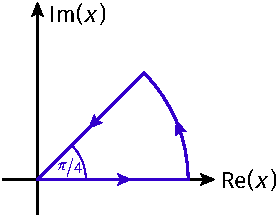
\includegraphics[width=\textwidth]{fresnel}

   \vspace{-0.4truecm}
  \end{column}
 \end{columns}
\end{frame}

\begin{frame}[c]{Propagator of a free particle and\\ relation to classical properties}
 propagator 
 \begin{displaymath}
  K(q_\text{f}, q_\text{i}, t) = \langle q_\text{f}\vert\text{e}^{-\frac{\text{i}}{\hbar}Ht}
                                   \vert q_\text{i}\rangle
     = \sqrt{\frac{m}{2\pi\text{i}\hbar t}}\exp\left(\frac{\text{i}}{\hbar}
	    \frac{m(q_\text{f}-q_\text{i})^2}{2t}\right)
 \end{displaymath}

 \vspace{0.3truecm}
 classical motion from position $q_\text{i}$ to $q_\text{f}$ in time $t$:
 \begin{itemize}
  \item classical path\quad $q(s) = q_\text{i} + (q_\text{f}-q_\text{i})\dfrac{s}{t}$
  \item classical action\quad
	$S_\text{cl} = \int_0^t\text{d}s\dfrac{m}{2}\dot q^2
		     = \dfrac{m(q_\text{f}-q_\text{i})^2}{2t}$
 \end{itemize}

 \vspace{0.4truecm}
 propagator of free particle in terms of classical properties

 \begin{center}
  \fcolorbox{red!70!black}{red!10}{\alert{%
  $K(q_\text{f}, q_\text{i}, t) = \sqrt{-\dfrac{1}{2\pi\text{i}\hbar}
	 \dfrac{\partial^2 S_{cl}}{\partial q_\text{i}\partial q_\text{f}}}
	 \exp\left(\dfrac{\text{i}}{\hbar}S_\text{cl}\right)$
  }}
 \end{center}
\end{frame}

\begin{frame}[c]{Combining two propagators}
 \begin{displaymath}
  \begin{aligned}
   K(q_\text{f}, q_\text{i}, t_2+t_1) &= \langle q_\text{f}\vert
	  \text{e}^{-\frac{\text{i}}{\hbar}Ht_2}
	  \text{e}^{-\frac{\text{i}}{\hbar}Ht_1}\vert q_\text{i}\rangle\\
     &= \textcolor{blue}{\int_{-\infty}^{+\infty}\text{d}q'}\langle q_\text{f}\vert
	  \text{e}^{-\frac{\text{i}}{\hbar}Ht_2}\textcolor{blue}{\vert q'\rangle\langle q'\vert}
	  \text{e}^{-\frac{\text{i}}{\hbar}Ht_1}\vert q_\text{i}\rangle\\
     &= \int_{-\infty}^{+\infty}\text{d}q' K(q_\text{f}, q', t_2)K(q', q_\text{i}, t_1)
  \end{aligned}
 \end{displaymath}

\end{frame}

\section{Derivation of path integral}

\begin{frame}[c]{}
 \begin{center}
  \begin{minipage}{0.8\textwidth}
   \tableofcontents[currentsection]
  \end{minipage}
 \end{center}
\end{frame}

\begin{frame}[t]{}
\end{frame}

\section{Particle in a box}

\begin{frame}[c]{}
 \begin{center}
  \begin{minipage}{0.8\textwidth}
   \tableofcontents[currentsection]
  \end{minipage}
 \end{center}
\end{frame}

\begin{frame}[t]{}
\end{frame}

\section{Particle on a ring}

\begin{frame}[c]{}
 \begin{center}
  \begin{minipage}{0.8\textwidth}
   \tableofcontents[currentsection]
  \end{minipage}
 \end{center}
\end{frame}

\begin{frame}[t]{}
\end{frame}

\section{Harmonic oscillator}

\begin{frame}[c]{}
 \begin{center}
  \begin{minipage}{0.8\textwidth}
   \tableofcontents[currentsection]
  \end{minipage}
 \end{center}
\end{frame}

\begin{frame}[t]{}
\end{frame}
\end{document}
